
\documentclass[ms.tex]{subfiles}
\begin{document}

\section{Observational Diagnostics}
\label{sec:diagnostics}

Due to the redshift evolution of the MZR, the mass dependence of the specific
SN Ia rate at different redshifts could empirically distinguish between
$\gamma = 0$ and~$\gamma = -0.5$.
To investigate this possibility, we take the same~$z = 0$ stellar masses
spanning~$10^{7.2} - 10^{12}~\msun$ and determine their corresponding stellar
masses at redshifts of~$z = 0.5$ and~$1$ by evaluating equation~\refp{eq:specia}
up to~$T = 13.2$ Gyr from the appropriate lookback time as opposed to zero for
the present day (we assume the cosmological parameters measured from the cosmic
microwave background in~\citealt{Planck2014} and compute the lookback times
using~\textsc{Astropy}).
We additionally compute the implied stellar mass for the appropriate redshift
(i.e. the denominator of equation~\ref{eq:specia}) and use that value to
evaluate the~\citet{Zahid2014} MZR to compute metallicity-dependent rates with
$\gamma = -0.5$.
To compare to a case where~$\gamma = 0$, we omit the~$\gamma = -0.5$ correction
and instead apply an additional~$(M_\star / 10^{10} \msun)^{-0.15}$
prefactor to account for the shallower mass dependence.
This prefactor brings the~$\gamma = 0$ case into better agreement with the
$\gamma = -0.5$ case at~$z = 0$ and is intended to encapsulate the otherwise
unknown processes which amplify the SN Ia rate at low stellar masses if it is
instead not due to metallicity effects.
We nonetheless caution that this is a purely~\textit{a posteriori} correction
not based on physical arguments so that we can make an ``apples to apples''
comparison between two models which agree with an~$M_\star^{-0.3}$ scaling at
$z = 0$ as suggested by~\citet{Gandhi2022}, and it does not include any
potential redshift-dependence in the unknown processes.
\par
We plot the resulting specific SN Ia rates as a function of stellar mass at
$z = 0$,~$0.5$ and~$1$ in Fig.~\ref{fig:specia_zdep}.
In both the~$\gamma = 0$ and $\gamma = -0.5$ cases, the scaling of the specific
SN Ia rate with galaxy stellar mass becomes shallower with increasing redshift.
If~$\gamma = -0.5$, these calculations suggest that it should decrease by a
factor of~$\sim$2 between~$z = 0$ and~$z = 1$ at~$\mstar \approx
10^{7.2}~\msun$, the lowest stellar mass for which we have made predictions at
all three redshifts.
If~$\gamma = 0$, then the rate instead decreases by a factor of~$\sim$3 at
$\sim 10^{7.2}~\msun$.
This difference arises because the metallicities of dwarf galaxies decrease
with increasing redshift and~$\gamma = -0.5$ allows them to sustain higher
SN Ia rates than if~$\gamma = 0$.
Distinguishing between these models empirically, however, would require a
considerably precise SMF at redshift~$z = 1$.
Factors of 2 and 3 between~$10^{7.2}$ and~$10^{10}~\msun$ are produced by
power-law indeces of~$-0.108$ and~$-0.170$, respectively. 
The difference between the two ($0.062$) is the minimum precision required
on the slope of the SMF at the low-mass end, only slightly larger than the
precision achieved by~\citet[][$\pm 0.05$, see their Fig. 13]{Baldry2012}.
Therefore, this empirical test requires at least their level of precision but
at~$z \approx 1$.
\par
Although current surveys lack the depth required to pin down SN rates across
multiple decades of stellar mass at~$z = 1$, the sample sizes necessary to do
so may be feasible with next-generation facilities.
First and foremost, the Nancy Grace Roman Space Telescope (\citealp{Spergel2013,
Spergel2015}; formerly the Wide Field Infrared Survey Telescope -- WFIRST),
among other motivations, was designed for exactly this purpose in order to
constrain the dark energy equation of state using high-redshift SNe Ia.
The Roman~\textit{H} band in particular has excellent prospects for discovering
all classes of SNe at redshifts as high as~$z \gtrsim 2$ and beyond
\citep{Petrushevska2016}.
The 6.6-meter aperture of the recently-launched James Webb Space Telescope
\citep[JWST;][]{Gardner2006} will provide sensitivity as low as the~$\sim$31st
magnitude in the optical and mid-infrared, sufficient to discover SNe as
distant as~$z \gtrsim 4$.
Stellar masses can then be derived for the host galaxies which have
spectroscopic information available from, e.g., JWST itself or the Dark Energy
Spectroscopic Instrument~\citep[DESI;][]{Desi2016}.
However, the resultant constraints on the specific SN Ia rate as a function of
stellar mass will require precise nkowledge of how the SMF varies with redshift.
Such measurements are challenging with current galaxy samples from, e.g.,
SDSS due to their flux-limited nature and the broad range of mass-to-light
ratios spanned by galaxies~\citep{Weigel2016}.
State-of-the-art facilities like DESI and JWST which have recently begun
collecting data should achieve significantly higher completeness for dwarf
galaxies at~$z \approx 1$ due to their higher sensitivities, but as discussed
above, achieving the level of precision required for this empirical test could
be challenging, even with these instruments.

\begin{figure}
\centering
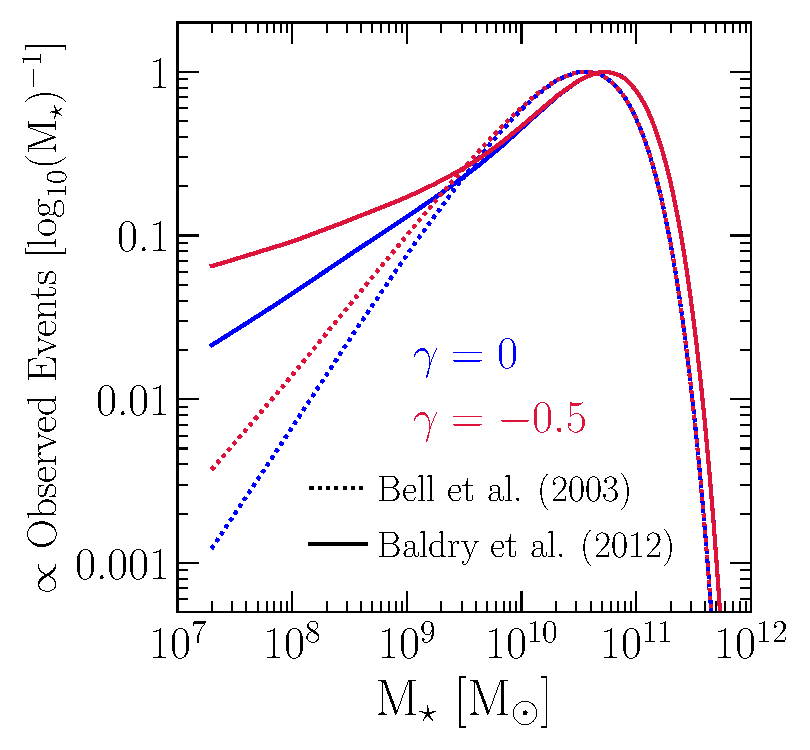
\includegraphics[scale = 0.55]{ia_massdist.pdf}
\caption{
The predicted stellar mass distribution of SN Ia host galaxies in an
untargeted survey (see equation~\ref{eq:hostmassdist}) with the
\citet[][dotted]{Bell2003} and~\citet[][solid]{Baldry2012} SMFs combined with
both metallicity dependent ($\gamma = -0.5$, red) and metallicity independent
rates ($\gamma = 0$, blue).
All distributions are normalized to a maximum value of 1.
}
\label{fig:hostmassdist}
\end{figure}

While empirical measurements of the specific SN Ia rate as a function of
stellar mass depend on the assumed SMF~\citep{Gandhi2022}, the host galaxy
mass distribution of observed events does not, making it a potentially more
observationally feasible diagnostic.
As noted in Fig.~\ref{fig:specia_metdep}, only dwarf galaxies are
significantly affected by a metallicity-dependent scaling of SN Ia rates due to
the shape of the MZR, so a~$\gamma \approx -0.5$ scaling should present as an
enhanced tail at the low-mass end of the distribution.
Although this empirical measurement does not depend on the SMF, our theoretical
prediction does because we must take into account the relative abundances of
galaxies of different stellar masses.
The observed rate in a bin of stellar mass can be expressed as the product
of the characteristic rate~$\dot{N}_\text{Ia}$ at a given stellar mass and
the integral of the SMF~$\Phi(M_\star)$ over the bin in stellar mass according
to
\begin{equation}
\dot{N}_\text{Ia,cosmic}(M_\star | \gamma) = \dot{N}_\text{Ia}(M_\star | \gamma)
\int_{M_\star}^{M_\star + dM_\star} \Phi(M_\star) dM_\star,
\label{eq:hostmassdist}
\end{equation}
where~$\dot{N}_\text{Ia}$ is given by the numerator of
equation~\refp{eq:specia}.
We plot this distribution in Fig.~\ref{fig:hostmassdist} for each combination
of~$\gamma = 0$ and~$-0.5$ with the SMFs parametrized by~\citet{Bell2003}
and~\citet{Baldry2012} in logarithmically spaced bins of stellar mass,
normalizing to a maximum value of 1 in all cases.
For untargeted surveys like ASAS-SN, equation~\refp{eq:hostmassdist} should
describe the observed host galaxy stellar mass distribution exactly, whereas
targeted surveys like the Lick Observatory SN Search~\citep[LOSS;][]{Li2000,
Filippenko2001} would be impacted by selection criteria.
\par
According to this formalism, galaxies with stellar masses of
$M_\star \approx 3-5 \times10^{10}~\msun$ should dominate the detected SN Ia
events for all choices of the SMF and~$\gamma$.
This peak arises as the optimal stellar mass which is high enough to produce a
large number of WDs, but being near the ``knee'' of the SMF, is not so high
that the galaxies themselves are rare.
For a given choice of the SMF, $\gamma = -0.5$ indeed enhances the low-mass
tail of the distribution, increasing the number of observed SN Ia events in
$M_\star \approx 10^{7.2}~\msun$ galaxies by a factor of~$\sim$3 relative to
$\gamma = 0$.
However, Fig.~\ref{fig:hostmassdist} indicates that this observed distribution
is a considerably better diagnostic of the SMF itself as opposed to the
metallicity dependence of SN Ia rates or lack thereof.
Between the position of the peak and~$10^{7.2}~\msun$, the host mass
distribution computed with the~\citet{Bell2003} SMF drops by~$\sim$2.5 orders
of magnitude while that computed with the~\citet{Baldry2012} SMF drops
by~$\sim$1.5 orders of magnitude.
Nonetheless, once precise knowledge of the SMF -- independent of SN rates -- is
available, this diagnostic could distinguish between different models for the
metallicity dependence of SN Ia rates.

\end{document}
